% ============================================================================
% Paper F — Calibrated online readout and sparse selectivity on an SSM host
%   Companion to Paper D (REDEM-SSM diagnostics).
% Target: Neurocomputing / TMLR (mechanism + methodology; honest negatives).
% Compile: pdflatex PAPER_F.tex (twice for cross-refs).
% Numbers: data/s50_*, s51_*, s52_* (10 seeds, s18/s19 paired protocol).
% ============================================================================
\documentclass[preprint,12pt]{elsarticle}

\usepackage{amsmath,amssymb}
\usepackage{booktabs}
\usepackage{graphicx}
\usepackage{url}
\usepackage{lmodern}
\usepackage{microtype}
\setlength{\emergencystretch}{1em}

\graphicspath{{../figures/}}

\journal{Neurocomputing}

\begin{document}

\begin{frontmatter}

\title{Learning the Readout Form: Objective-Level Calibration, Sparse
Selectivity, and Expert Routing on a Diagonal State-Space Host}

\author[a]{Yaming Hu\corref{cor1}}
\cortext[cor1]{Corresponding author. ORCID: 0009-0003-1406-0485.}
\ead{64687555@qq.com}
\address[a]{Independent Researcher, Guiyang, Guizhou, China}

\begin{abstract}
Online adaptation on a state-space host is often judged with a
human-specified output form. We show that this choice is load-bearing.
On the same diagonal SSM host and paired stream protocol as Paper~D, a
squared-loss RLS readout
evaluated with a clip floor parks $1.6$--$10.2\%$ of tokens on a
fixed floor; several stream comparisons become floor-sensitive.
Replacing the evaluation---not the numeric range---with a
trained softmax readout removes the floor and
lowers stream cross-entropy by $0.307$~nats/token (perplexity
$11.75\to8.65$, $10/10$ seeds), at a retention cost of $+0.32$
same-token-set ppl ($1/10$). A post-hoc simplex projection that
removes all negatives does \emph{not} repair the metric
(stream $\Delta$ppl $+0.03$, $0/10$): the artifact lives in the
objective, not the range. Under the clean metric the ungated full
state remains stream-neutral and retention-harmful; a $128$-dimensional
noise control rules out dimension/optimizer imbalance, while a
$32$-dimensional state slice is stream-positive. Unconstrained
cross-entropy training of a feature-level gate improves stream form
but does not sparsify and destroys retention. Hard top-$k$ sparsity
($k=32$) is the missing pressure: it yields the best stream arm
($7.03$) at near-baseline retention. Soft routing over two online
softmax experts reduces forgetting further ($9.20\to7.79$,
$10/10$) at stream parity; a hard-routing ablation is slightly better
on retention ($6.94$) at a small stream tax. The full stack beats the calibrated
input-path baseline on both axes. We state a design rule---the
evaluation instrument must be part of the learned system---and the
boundary where it stops paying: candidate-family breadth remains
human-supplied. All results are CPU-scale; we make no scaling or
state-of-the-art claims.
\end{abstract}

\begin{keyword}
online learning \sep
state-space models \sep
readout calibration \sep
selective state space \sep
continual learning \sep
falsification
\end{keyword}

\end{frontmatter}

\section{Introduction}
\label{sec:intro}

Self-correcting learning systems are usually evaluated with
instruments the designer fixed in advance: a loss, a readout
parameterization, a scoring rule. When those instruments are part of
what training changes, evaluation and improvement can share a
gradient. When they are frozen and human-prescribed, the system
optimizes a different quantity than the one used to judge it, and
artifacts of that mismatch can survive any amount of downstream
``self-correction.''

Paper~D (companion; \cite{dpaper}) diagnosed a diagonal state-space host under such a
prescribed instrument: per-token recursive least squares (RLS) on a
linear readout, scored as
$\mathrm{CE}=-\ln\mathrm{clip}(\hat y_t[e_t],10^{-12},1)$.
That work established a deconvolution impossibility for recovering the
current token from a linearly decayed state mixture, identified the
additive input path as required for calibration, and showed that
several stream rankings reverse once clipped tokens are excluded.
Paper~E, on a different substrate, measured the complementary
ceiling at the decision layer: under a $\pm1$ reward channel,
autonomy reduces to selection among a human-supplied pair of
correction laws.

This paper is written \emph{as the rule} extracted from those traps.
We keep Paper~D's host, task, and seed rules so that every row pairs
bitwise with the diagnostics, and we change what is allowed to be
learned:

\begin{enumerate}
\item \textbf{C1 (objective, not range).} A trained softmax readout
removes the clip floor and lowers stream CE by $0.307$~nats/token
(ppl $-26\%$), with an honest retention cost in the same sentence.
\item \textbf{C2 (post-hoc control).} Projecting the same RLS solution
onto the probability simplex after the fact eliminates all negatives
and does \emph{not} improve stream ppl ($0/10$). Range fixes are
decoration.
\item \textbf{C3 (boundary under a clean metric).} The ungated full
state is stream-neutral and retention-harmful; dimension and optimizer
imbalance are excluded by noise and width-matched controls.
\item \textbf{C4/C4b (learned sparse selectivity).} Unconstrained
cross-entropy training of a feature-level gate improves stream form
but does not sparsify and collapses retention. Hard top-$k$ sparsity
is the missing pressure: best stream at near-baseline retention.
\item \textbf{C5 (expert routing).} Soft routing over two online
softmax experts on the sparse-gated base reduces forgetting by
$1.41$~ppl ($10/10$) at stream parity.
\end{enumerate}

\paragraph{Feedback budget.}
Following the reporting discipline of Papers~D and~E, every autonomy
or form-discovery claim is stated together with the information the
system was allowed to see. Here the budget is \emph{per-token labels}
via cross-entropy---strictly richer than Paper~E's $\pm1$ channel. We
do not port Paper~E's decision-layer mechanism stack onto this host:
the reason those mechanisms exist (no gradient to a parameter) is
absent once a calibrated CE objective is available.

\paragraph{Claims we do not make.}
Proposition~1 of Paper~D is not ``beaten''; our gains come from
recalibrating the input path and from sparse gating, not from
inverting a linear deconvolution. We do not claim SOTA against
Mamba/TTT/DeltaNet, scaling, or multi-step RL. All results are
CPU-scale ($N=128$) on a two-domain biased-bigram stream.

\section{Related work}
\label{sec:related}

\paragraph{Online learning inside sequence models.}
Test-time training and related ideas update hidden representations or
readouts at inference~\cite{sun2024ttt}. Linear-recurrence and
selective SSM architectures provide a host whose state can be updated
online~\cite{sun2024ttt,gu2023mamba,gu2022s4}; fixed random reservoirs
with trained readouts are the classical online-readout
substrate~\cite{jaeger2001,lukosevicius2009}.
Paper~D positioned an explicit
per-token RLS readout and REDEM mechanism division of labor against
amortized online learners and surprise-based memories; parameter-efficient
adapters such as LoRA~\cite{hu2022lora} are the usual amortized reference.
We inherit the host and change only the readout form and selectivity
pressure.

\paragraph{Metric artifacts in online CE.}
Clipped linear scores on squared-loss readouts create a floor mass
that can drive stream rankings. Paper~D reported clip fractions and
unclipped sensitivity analyses. This paper adds the missing control:
a post-hoc range fix (simplex) versus an objective fix (trained
softmax).

\paragraph{Sparse and gated features.}
Hard cardinality constraints (top-$k$) and $\ell_1$ pressures are
standard tools for feature selection. Our use is online and coupled
to a recurrent host: the gate multiplies whitened state channels while
the current-token input path stays clean---the additive path that
Paper~D showed is required.

\paragraph{Mixture of experts online.}
Soft mixtures of specialists with responsibility-weighted updates are
classical. Here experts are \emph{online softmax readouts} selected by
a fast-channel EMA domain statistic (Paper~D's M3 metadata), under a
clean metric, on a sparse-gated state slice. Catastrophic-forgetting
baselines such as EWC~\cite{kirkpatrick2017} and consolidation accounts
of multi-timescale memory~\cite{benna2016} are not the focus here
(Paper~E reports a matched-optimizer negative); we stay inside the
readout-form question.

\section{Preliminaries: host, metric, and Paper~D's boundary}
\label{sec:prelim}

\subsection{Diagonal SSM host}
Following Paper~D,
\begin{equation}
h_t = A\odot h_{t-1} + B e_{t-1},\qquad
A=\mathrm{diag}\big(\exp(-1/\tau_i)\big),
\end{equation}
with log-uniform $\tau_i\in[1,3000]$ and spectrum whitening
$h^w_t = h_t\odot\sqrt{N(1-A_i^2)}$, $N=128$.
The additive input path $x_t=B e_{t-1}$ is retained as a clean feature
(D: the current token cannot be recovered from the linearly mixed
state by a linear readout).

\subsection{Clipped-linear metric (Paper~D)}
Squared-loss RLS on $\phi$ produced $\hat y=W\phi$, scored as
\begin{equation}
\mathrm{CE}=-\ln\mathrm{clip}(\hat y[e_t],10^{-12},1),
\end{equation}
The input-path arm parks $\sim1.6\%$ of stream tokens on the floor;
state-feature arms park $\sim10\%$. Paper~D showed rankings that
reverse under unclipped sensitivity metrics and scoped several stream
claims as floor-sensitive.

\subsection{What this paper changes}
We treat the readout \emph{map} and the \emph{gate form} as trainable
objects under a proper probabilistic objective, and we ship the
post-hoc simplex arm next to every headline (Section~\ref{sec:exp}).

\section{Method}
\label{sec:method}

\subsection{C1: trained probabilistic readout}
Let $\phi_t$ be any feature concatenation ending with a bias. We
predict
\begin{equation}
p_t=\mathrm{softmax}(W\phi_t),\qquad
\mathcal{L}_t=-\ln p_t[e_t],
\end{equation}
and update $W$ with AdaGrad (lr $0.05$, gradient clip $5.0$; plain SGD
exploded on high-dimensional skip features). Softmax outputs are
strictly positive; $\texttt{floor\_frac}=0$ is true by construction and
is never quoted as an empirical finding.

\subsection{C2: post-hoc simplex control}
As a control, we keep RLS training on squared error and only change
the evaluation map to
$\Pi_\Delta(\hat y)=\max(\hat y,0)/\sum_j\max(\hat y_j,0)$ (uniform
fallback if the mass vanishes). This is clip-negatives plus
renormalize --- not a Euclidean projection onto the probability simplex
--- and it removes every negative score without changing the learned $W$.

\subsection{C4b: sparse learned gate}
\begin{equation}
g_t=\mathrm{TopK}_k\big(\sigma(C x_t+b)\big),\qquad
\phi_t=\big[\,h^w_t\odot g_t;\; x_t;\; 1\,\big],
\end{equation}
with $k=32$ matched to the width of the best fixed state slice. $C,b$
are trained jointly with the readout under the same CE objective;
non-selected channels receive zero gradient through the gate (straight
through the hard mask). An $\ell_1$ variant is reported as an ablation.

\subsection{C5: soft expert routing}
Fast-channel EMA metadata (Paper~D M3; $\tau_i\le 8$, $\tau_m=500$)
yields $m_t$ and fixed per-domain references. Soft routing uses
\begin{equation}
\pi_{t,k}=\mathrm{softmax}_k\big(-\|m_t-\mathrm{ref}_k\|/T_r\big),\quad
p_t=\sum_k \pi_{t,k}\,\mathrm{softmax}(W_k\phi_t),
\end{equation}
with exact mixture responsibility
$\pi_{t,k}\,p_{t,k}[e_t]/p_t[e_t]$ scaling each expert's CE gradient.
Hard nearest-reference routing (Paper~D A3 semantics) is an ablation.
Holdout evaluation of each expert uses a single-step EMA of the
matching domain reference (same metadata path as stream); this is
disclosed here because it injects domain identity at evaluation time
and is not a fully blind holdout.

\section{Experiments}
\label{sec:exp}

\subsection{Protocol}
Task and seeds are verbatim from Paper~D / s18: two biased-bigram
Markov domains alternating every $3000$ tokens, $6$ segments, $10$
seeds, seed rule $\mathrm{seed}\times101+17$. The control arm
\texttt{B-lin-clip} reproduces Paper~D's \texttt{B-proj} stream,
forgetting, and clip fraction exactly ($\max|\Delta|=0$ on all three
metrics, $10/10$). Forgetting is the held-out previous-domain
perplexity of the final readout (domain-matched specialist when
routing). Head-to-head statements use same-token-set CE where
relevant. We report means over seeds and sign counts; we do not merge
\texttt{clip\_frac} with \texttt{floor\_frac}.

\subsection{C1--C2: readout form}
\begin{table}[h]
\centering
\caption{Readout form (10-seed means). Post-hoc simplex removes
negatives ($\texttt{neg\_frac}\to0$) but does not repair stream ppl
(C2). Trained softmax does (C1), with a small retention cost.}
\label{tab:c1c2}
\begin{tabular}{lcccc}
\toprule
Arm & stream & forget & clip\% & floor\% \\
\midrule
B-lin-clip (D B-proj) & 11.754 & 8.387 & 1.58 & -- \\
B-simplex (post-hoc) & 11.783 & 8.387 & 0 & 1.58 \\
\textbf{B-softmax-sgd} & \textbf{8.648} & 8.890 & 0 & 0$^\dagger$ \\
Skip-lin-clip (D CV-skip) & 58.465 & 94.057 & 10.23 & -- \\
Skip-simplex & 75.736 & 140.234 & 0 & 10.23 \\
Skip-softmax-sgd & 8.629 & 57.711 & 0 & 0$^\dagger$ \\
\bottomrule
\end{tabular}
\end{table}

Same-token-set stream: B-softmax vs B-lin-clip $\Delta$CE $=-0.307$
($10/10$; paired $t=-92.3$ from an offline seed-level reduction of the
committed per-token CE arrays, not a separate script);
B-simplex vs B-lin-clip $\Delta$ppl $=+0.03$
($0/10$). Retention price of C1: same-set $\Delta$ppl $+0.32$
($1/10$). The range-fix story is visualized in
Figure~\ref{fig:floor}: the post-hoc simplex relocates the clipped
negative mass to the floor, while the trained softmax removes it by
construction.

\begin{figure}[ht]
\centering
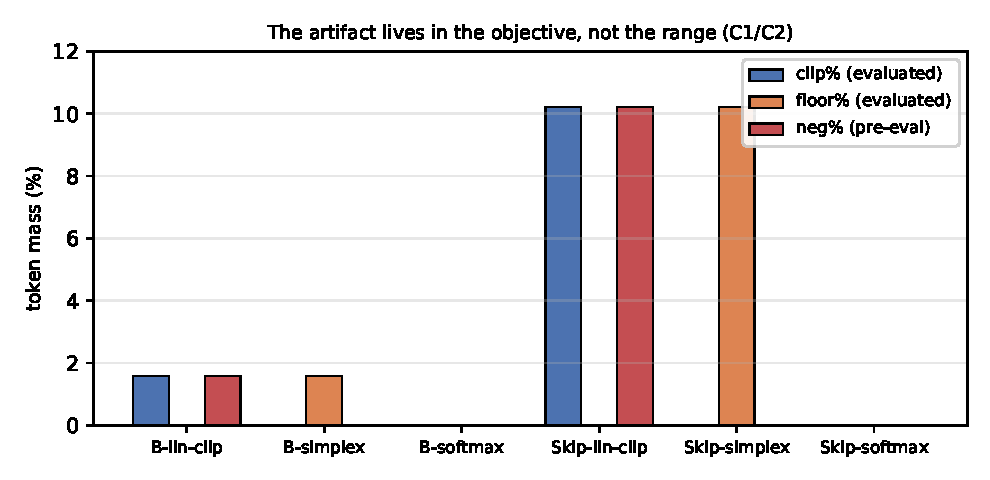
\includegraphics[width=0.92\textwidth]{paperF_fig2_floor}
\caption{Clip-floor artifact across readout forms (10-seed means).
Negatives under the clipped-linear metric (\texttt{neg\_frac}) are
parked on the floor by clipping (\texttt{clip\_frac}); the post-hoc
simplex arm relocates that mass to \texttt{floor\_frac} without
improving stream ppl (C2). The trained softmax readout has none of
either by construction (C1).}
\label{fig:floor}
\end{figure}

\subsection{C3: state under a clean metric}
\begin{table}[h]
\centering
\caption{Dimension/optimizer controls under softmax (10-seed means).}
\label{tab:c3}
\begin{tabular}{lcc}
\toprule
Arm & stream & forget \\
\midrule
B-softmax-sgd & 8.648 & 8.890 \\
B-noise-softmax ($\varepsilon^{128}$) & 10.271 & 9.554 \\
Skip-sub-softmax ($h^w_{[:32]}$) & 8.142 & 11.231 \\
Skip-softmax-sgd (full $h^w$) & 8.629 & 57.711 \\
\bottomrule
\end{tabular}
\end{table}

B-softmax vs Skip-softmax: stream $\Delta$CE $+0.003$ ($t=0.22$);
forget $\Delta$CE $-1.348$ ($10/10$). Noise does not collapse
retention (dimension is not the cause). A $32$-dimensional slice is
stream-positive vs B-softmax ($\Delta$CE $+0.061$, $9/10$) with mild
retention cost.

\subsection{C4/C4b: learned selectivity and sparsity}
\begin{table}[h]
\centering
\caption{Gates under CE (10-seed means). Unconstrained Gate-C is the
best non-sparse stream arm but fails retention; top-$k$ fixes both.}
\label{tab:c4}
\begin{tabular}{lccc}
\toprule
Arm & stream & forget mean/med & notes \\
\midrule
Skip-sub & 8.142 & 11.231 / 9.908 & fixed slice \\
Gate-C & 7.741 & 31.075 / 26.155 & gate $\approx0.72$ open \\
\textbf{Gate-C-topk} & \textbf{7.033} & \textbf{9.201 / 9.330} & $k=32$ \\
Gate-C-L1 & 6.994 & 11.574 / 11.136 & $\lambda=0.01$ \\
\bottomrule
\end{tabular}
\end{table}

Gate-C-topk vs B-softmax: stream better $10/10$ ($-1.62$);
forget mean $+0.31$ ($3/10$ better) --- near parity. Gate-C-topk vs
Gate-C: forget better $10/10$ ($-21.9$). Cross-entropy alone does not
sparsify; hard cardinality is the pressure that turns selectivity into
a retention-safe mechanism.

\subsection{C5: expert routing}
\begin{table}[h]
\centering
\caption{Routing on the Gate-C-topk base, $\tau_m=500$ (10-seed means).}
\label{tab:c5}
\begin{tabular}{lccc}
\toprule
Arm & stream & forget mean/med & $\Delta$forget vs Single \\
\midrule
Single-topk & 7.033 & 9.201 / 9.330 & -- \\
\textbf{Soft-topk} & 7.065 & \textbf{7.789 / 7.717} & $-1.41$ ($10/10$) \\
Hard-topk & 7.111 & 6.939 / 6.913 & $-2.26$ ($10/10$) \\
\bottomrule
\end{tabular}
\end{table}

Soft vs Single stream $\Delta$CE mean $+0.03$ ($t=0.68$) --- parity.
Hard pays a small stream tax for stronger retention (Paper~D's
specialization--lag tradeoff survives under a calibrated readout).
\textbf{Full stack vs B-softmax}: Soft-topk stream $7.065$ vs
$8.648$; forget $7.789$ vs $8.890$ --- both axes better.
Figure~\ref{fig:arms} summarizes the headline arms across C1--C5 on
both axes (10-seed means $\pm$ std).

\begin{figure}[ht]
\centering
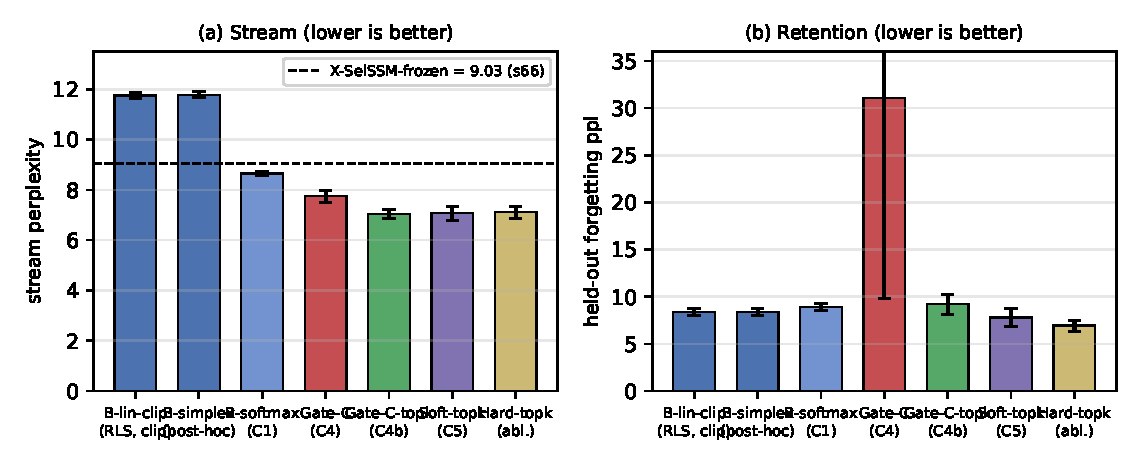
\includegraphics[width=\textwidth]{paperF_fig1_arms}
\caption{Headline arms across C1--C5 (10-seed means $\pm$ std).
(a) Stream perplexity: the trained softmax readout (C1) removes the
clip floor and improves stream; hard top-$k$ gating (C4b) is the best
stream arm and sits below the frozen selective-SSM reference (dashed
line, s66). (b) Held-out forgetting: the unconstrained gate (C4)
collapses retention, top-$k$ restores parity, and soft expert routing
(C5) converts the remaining stream--retention tension into a further
retention gain.}
\label{fig:arms}
\end{figure}

\section{Analysis}
\label{sec:analysis}

\paragraph{Why simplex fails and softmax works.}
RLS on squared error is free to drive the target coordinate
non-positive; clipping or projecting after the fact cannot restore
mass that the objective never placed on the simplex. Softmax CE
constrains the map during learning. C2 is therefore not a minor
ablation: it is what makes C1 a statement about objectives rather than
about numeric hygiene.

\paragraph{Why CE does not produce a sparse gate.}
Stream CE is largely satisfied by a moderately open gate that keeps
domain-level and mixture information; that same open gate is what
poisons held-out retention (C3). Sparsity must be imposed as a
constraint (top-$k$), not hoped for from the task loss.

\paragraph{Hard vs soft routing.}
Hard routing purer specialists (lower forget) at a lag cost on stream;
soft routing mixes and keeps stream at parity while still buying
$1.4$~forget. This mirrors Paper~D's soft-vs-abrupt finding under a
different readout family.

\paragraph{Design rule.}
\emph{Self-improvement requires a trustworthy self-evaluation, and the
instrument must be learnable rather than prescribed.} D prescribed the
readout form; E prescribed correction laws; F trains the form and
ships the post-hoc control that would have hidden the difference.

\section{Discussion}
\label{sec:discussion}

\paragraph{Feedback budget.}
All form-discovery results use per-token labels. They are not
comparable to $\pm1$ decision-layer autonomy without stating that
budget. We deliberately do not port Paper~E's mechanism stack: once a
gradient exists, the reason for a five-mechanism rule-selection tower
largely disappears, while retention must be re-measured under CE.

\paragraph{Boundary.}
Rules that make evaluation trustworthy do not generate new candidate
families. F learns form \emph{inside} supplied families (softmax maps,
gate parameterizations, expert mixtures). The next ceiling is
candidate-space \emph{breadth}: a trainable generator of hypotheses,
not only a scorer of human-supplied ones.

\paragraph{External baseline (s66) and the frozen-host surprise.}
{\sloppy
All s66 numbers cited below are $10$-seed means over the committed rows
of \url{data/s66_external_ssm_baseline_v1.json} (single
configuration: $N{=}128$ diagonal selective-SSM host on the char-level
biased-bigram stream; \texttt{stream\_ppl} is the stream perplexity and
\texttt{forgetting\_ppl} the held-out previous-domain perplexity; parameter
counts are the \texttt{n\_params\_readout}/\texttt{n\_params\_gate}/
\texttt{n\_params\_host} fields of the same file).
A Mamba-style selective-SSM arm on the identical host,
stream, seeds and metric does not close the gap to F's learned top-$k$
gate (stream $9.03$ vs.\ $7.03$, $0/10$ external better), and joint
online training of that external host is destructive. The more
informative observation is internal to the external pair: the
\emph{frozen} selective-SSM arm is the stronger external competitor
(stream $9.03$ vs.\ $10.19$; forget $10.38$ vs.\ $115.24$), yet it
still loses to F's calibrated softmax-sgd anchor on stream
($9.03$ vs.\ $8.65$) and on retention ($10.38$ vs.\ $8.89$). That
ordering --- random frozen selectivity $>$ jointly trained host ---
points to a pretrained-versus-random-host comparison, not to a claim
that selective SSMs are inferior in general. We therefore treat s66
as a scoped external check that licenses only the selective-SSM
parameterisation at this protocol scale.
}

\paragraph{Limitations.}
Two-domain biased-bigram stream; primary tables at $N=128$; one host
configuration. A Mamba-style selective-SSM baseline
(\texttt{s66}) has now been run on the same host, stream, seeds and
metric: the frozen-host external arm reaches stream ppl
(\texttt{stream\_ppl} mean) $9.03$ and the
jointly trained host arm is worse on both axes ($10.19$ stream at the
matched learning rate; retention collapses; a $4\times$ larger host
learning rate makes joint training diverge, so the committed
\texttt{s66} rows pool both rates under one arm name), while F's
learned top-$k$ gate remains best
($7.03$, $10/10$ paired seeds vs.\ the frozen external arm). The
external arm carries $\sim1.34\times$ the trainable parameters of
F's \emph{Gate-C-topk} arm ($33{,}088$ vs.\ $24{,}736$, from
\texttt{s66} committed rows: F's gate arm is readout ($8{,}224$) +
gate ($16{,}512$) $= 24{,}736$; the external arm is readout ($8{,}224$) +
host ($24{,}864$) $= 33{,}088$, fields
\texttt{n\_params\_readout}/\texttt{n\_params\_gate}/\texttt{n\_params\_host}),
so that gate win is not
a capacity fluke on this comparison; the ratio is not $1.34\times$ F's
ungated \texttt{B-softmax-sgd} anchor ($4{,}128$), against which the
external arm is much larger. This closes the earlier
``no external modern-SSM baseline'' gap for the
\emph{selective-SSM} family only --- one host configuration, one
protocol family, $N=128$, $10$ seeds, CPU scale; it is not a
state-of-the-art comparison and does not cover DeltaNet, gated linear
attention, or TTT (the TTT fast-weight arm scored worse than the
uniform predictor at this protocol scale and was removed as
non-viable). A width sweep
($N\in\{128,256,512\}$, 5 seeds) with $k=\max(8,N/4)$ showed the
calibrated input-path baseline improving with $N$ (stream
$8.63\to7.25$) while sparse-gate and soft-routing arms failed at
$N=512$ (Gate-C-topk stream $9.16$, forget $27.3$). A follow-up
$k$-sweep at $N=512$ (3 seeds) shows this is a \emph{sparsity}
failure, not a width impossibility: $k\in\{16,32\}$ restores the
ordering (Gate-C-topk $k=32$: stream $6.79$, forget $9.89$; Soft-topk
$k=16$: stream $6.59$, forget $6.27$) and beats the $N=512$
input-path baseline ($7.25$/$11.09$), whereas $k=128$ reproduces the
collapse. Claims should therefore be read as requiring a
\emph{fixed} modest $k$ (or a tuned $k(N)$), not $k\propto N$. A
Mackey-Glass bin-prediction task (5 seeds) supports transfer of the
sparse-gate advantage off the bigram stream (train/holdout ppl
$\approx20$/$16$ vs $30$/$29$ for the input-path baseline).
Softmax $\texttt{floor\_frac}=0$ is structural. These remain
proof-of-concept bounds.

\section{Conclusion}
\label{sec:conclusion}

Paper~D left a prescription: a calibrated output that removes the clip
floor, and learned selectivity as an open boundary. This paper ran the
prescription, falsified the post-hoc range fix, and showed that the
boundary only opens when selectivity is both \emph{learned} and
\emph{sparsity-pressured}, after which expert routing converts the
remaining stream--retention tension into a further retention gain. The
general lesson is narrower than ``use softmax'' and stronger than a
single mechanism: \textbf{put the evaluation instrument inside the
learned system}, and report the feedback budget next to every
autonomy claim.

\section*{Data and code}
CSVs and scripts under \texttt{data/} and \texttt{scripts/} (paired to
Paper~D \texttt{s19}/\texttt{s20}):
\begin{itemize}
\item \texttt{s50\_paper\_f\_pilot\_nl\_readout} (C1--C3);
\item \texttt{s51\_paper\_f\_learned\_gate} (C4/C4b);
\item \texttt{s52\_paper\_f\_soft\_route\_experts} (C5);
\item \texttt{s53\_paper\_f\_scaling} (width sweep);
\item \texttt{s53b\_paper\_f\_ksweep} ($k$-sweep at $N=512$);
\item \texttt{s54\_paper\_f\_mackey\_glass} (Mackey--Glass transfer);
\item \texttt{s66\_external\_ssm\_baseline} (selective-SSM baseline).
\end{itemize}

\section*{CRediT authorship contribution statement}
\textbf{Yaming Hu:} Conceptualization, Methodology, Software,
Validation, Formal analysis, Investigation, Data curation, Writing --
original draft, Writing -- review \& editing.

\begin{thebibliography}{9}

\bibitem{sun2024ttt}
Y.~Sun, X.~Li, K.~Dalal, J.~Xu, A.~Vikram, G.~Zhang, Y.~Dubois,
X.~Chen, X.~Wang, S.~Koyejo, T.~Hashimoto, and C.~Guestrin,
Learning to (Learn at Test Time): RNNs with Expressive Hidden States,
in Proc.\ of the 42nd Int.\ Conf.\ on Machine Learning (ICML),
PMLR 267:57503--57522, 2025.
% arXiv:2407.04620 — author list verified against the ICML/PMLR record

\bibitem{gu2023mamba}
A.~Gu, T.~Dao,
Mamba: Linear-Time Sequence Modeling with Selective State Spaces,
arXiv:2312.00752, 2023.

\bibitem{gu2022s4}
A.~Gu, K.~Goel, C.~R\'e,
Efficiently Modeling Long Sequences with Structured State Spaces,
ICLR, 2022.
% arXiv:2111.00396

\bibitem{jaeger2001}
H.~Jaeger,
The ``echo state'' approach to analysing and training recurrent neural
networks,
GMD Report 148, 2001.

\bibitem{benna2016}
M.~K. Benna, S.~Fusi,
Computational principles of synaptic memory consolidation,
Nature Neuroscience, 2016.

\bibitem{dpaper}
Y.~Hu,
REDEM-SSM: A State-Space Architecture with Native Online Learning,
Meta-Adaptation, and Structural Plasticity,
companion manuscript (Paper~D).

\bibitem{lukosevicius2009}
S.~Lukosevicius, H.~Jaeger,
Reservoir computing approaches to recurrent neural network training,
Computer Science Review, 2009.

\bibitem{kirkpatrick2017}
J.~Kirkpatrick, et al.,
Overcoming catastrophic forgetting in neural networks,
PNAS, 2017.

\bibitem{hu2022lora}
E.~J.~Hu, et al.,
LoRA: Low-Rank Adaptation of Large Language Models,
arXiv:2205.13098, 2022.

\end{thebibliography}

\section*{Declaration of competing interest}

The author declares no known competing financial interests or personal
relationships that could have appeared to influence the work reported in
this paper.

\section*{Funding}

This research did not receive any specific grant from funding agencies in
the public, commercial, or not-for-profit sectors.

\section*{Declaration of generative AI and AI-assisted technologies in
the writing process}

During the preparation of this work the author used language tools only
for language polish and code formatting. No scientific claims, data, or
figures were generated by AI. The author reviewed and edited all content
as needed and takes full responsibility for the paper.

\end{document}
